\chapter{Experiments with Real Aerial Data}
\section{Equipment Setup and Data Collection}
% word checked.
The biggest contribution of the project is that the algorithm was
tested and proven feasible with real flight data. The aerial video and
navigation data were collected through a survey flight with the
support of Sander Geophysics Ltd. A main purpose of the test flight is
to obtain aerial video with the camera close to the ground
to mimic the scenario of a low flying UAV. This is difficult to
achieve with any manned fixed wing aircraft. Therefore a simulated
unmanned aircraft system (SUAS) was used to carry all sensors. The
SUAS was towed by a helicopter via a tow rope of 33 meters long
(Figure \ref{fig:towedSUAS}). Yet, to prevent
the SUAS from being caught by tree branches, sufficient clearance must be
established between the SUAS and the vegetation. As a result, the helicopter
flew a planned path at approximately 100 meters above ground, and the SUAS
was at approximately 70 meters above ground.

\begin{figure}[h]
\centering
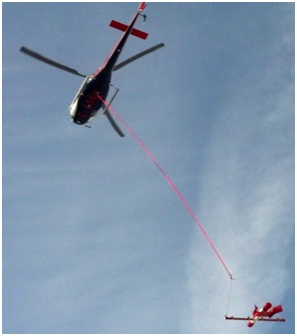
\includegraphics[width=5cm,keepaspectratio=true]{./Figures/towed_SUAS.jpg}
\caption{Simulated UAS towed by helicopter}
\label{fig:towedSUAS}
\end{figure}
\FloatBarrier

Sensors mounted on the SUAS included one wide angle CCD camera with
6mm focal length lens capturing monocular image sequence at 30 fps, a
pair of narrow angle CCD cameras for binocular images, one GPS
antenna, and one flight control INS/GPS navigation unit Athena 111m
\cite{_athena_????} (Figure \ref{fig:SUAS}). Analog video and
navigation data were sent to the helicopter via three BNC cables and
one data cable for recording. Installed in the helicopter are two SGL
data acquisition system CDAC. This system records video and navigation
data from the SUAS, as well as data from sensors installed on the
helicopter, including GPS, radar, laser altimeter, air pressure,
temperature, humility, etc. (figure \ref{fig:CDAC}). Videos from the
three cameras were digitized to a resolution of 720 pixels by 480
pixels using an MPEG4 video encoder from Parvus. The video was
time-stamped with GPS second on the image screen for post-flight
synchronization with the navigation data. A snapshot of the digitized
video is shown in figure \ref{fig:video_snapshot}.

\begin{figure}[h]
  \centering
  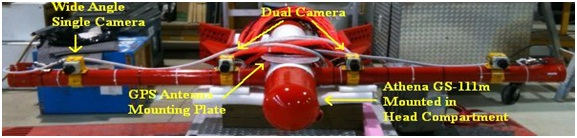
\includegraphics[width=14cm,keepaspectratio=true]{./Figures/SUAS.jpg}
  \includegraphics[width=6cm,keepaspectratio=true]{./Figures/athena.jpg}
  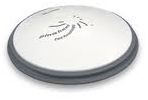
\includegraphics[width=6cm,keepaspectratio=true]{./Figures/GPS_antenna.jpg}
  \caption{Sensors mounted on SUAS. Top: the SUAS, bottom left: Athena
  GS-111m, bottom right: GPS antenna}
  \label{fig:SUAS}
\end{figure}

\begin{figure}[h]
  \centering
  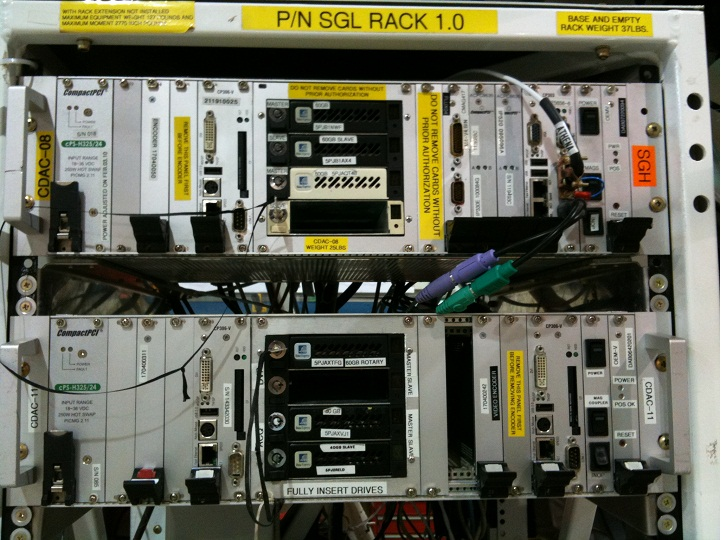
\includegraphics[width=12cm,keepaspectratio=true]{./Figures/CDAC_Rack.jpg}
  \caption{Compact PCI data acquisition system (CDAC)}
  \label{fig:CDAC}
\end{figure}

\begin{figure}[h]
  \centering
  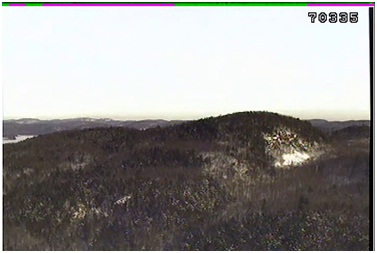
\includegraphics[width=12cm,keepaspectratio=true]{./Figures/video_snapshot.jpg}
  \caption{Image from monocular camera with GPS second timestamp}
  \label{fig:video_snapshot}
\end{figure}

\FloatBarrier

\section{Camera Calibration}\label{sec:camcal}
% word checked
A camera calibration was performed after the flight by taking a video
of a checker board pattern with various translation and rotation from
the camera. A total of 20 views of the calibration target were chosen
from the video, and fed to the calibration algorithm. A few examples
were shown in figure \ref{fig:camcal}.

\begin{figure}[h]
  \centering
  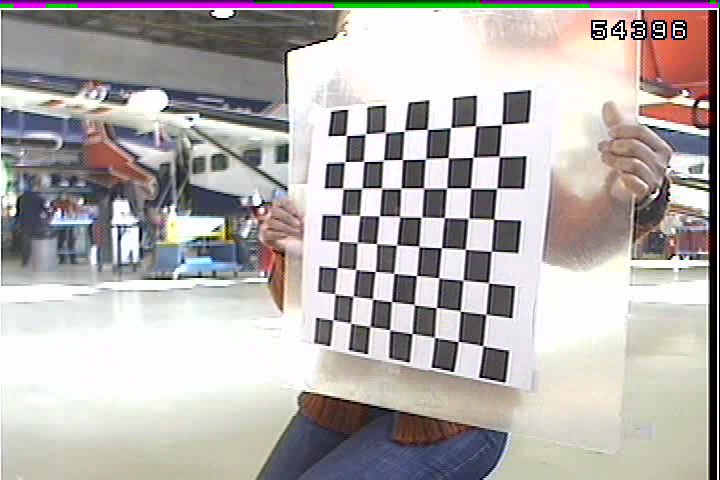
\includegraphics[width=4cm,keepaspectratio=true]{./Figures/camcal/camcal1_130.jpeg}
  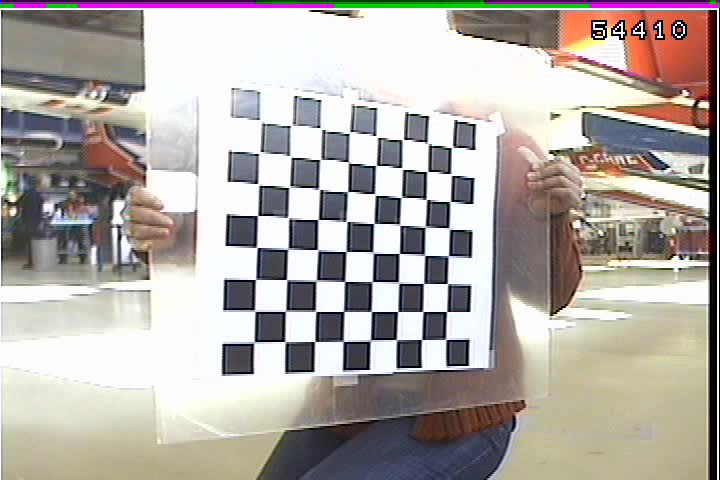
\includegraphics[width=4cm,keepaspectratio=true]{./Figures/camcal/camcal1_140.jpeg}
  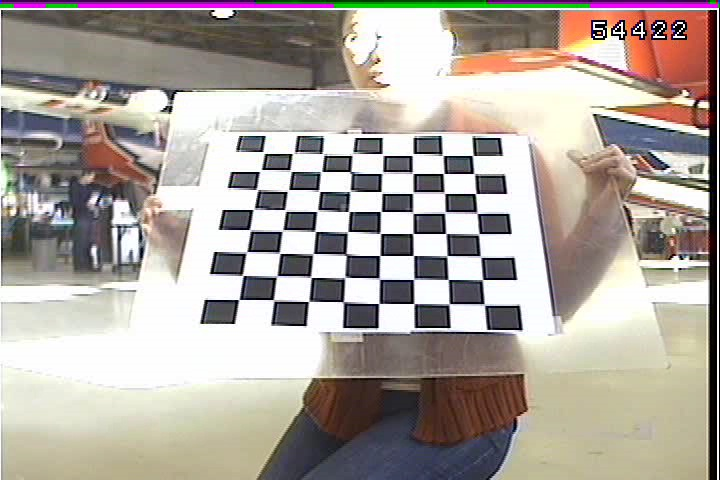
\includegraphics[width=4cm,keepaspectratio=true]{./Figures/camcal/camcal1_160.jpeg}
  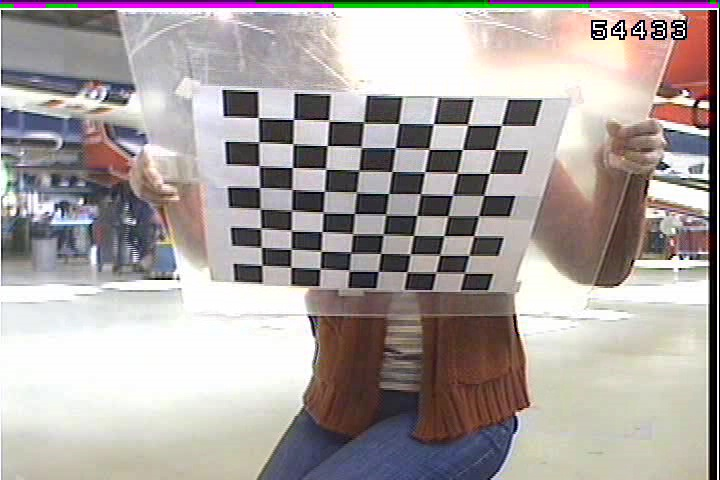
\includegraphics[width=4cm,keepaspectratio=true]{./Figures/camcal/camcal1_180.jpeg}
  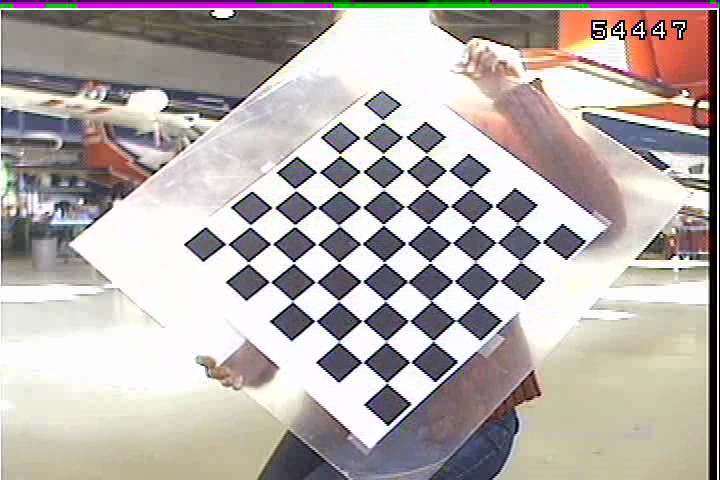
\includegraphics[width=4cm,keepaspectratio=true]{./Figures/camcal/camcal1_210.jpeg}
  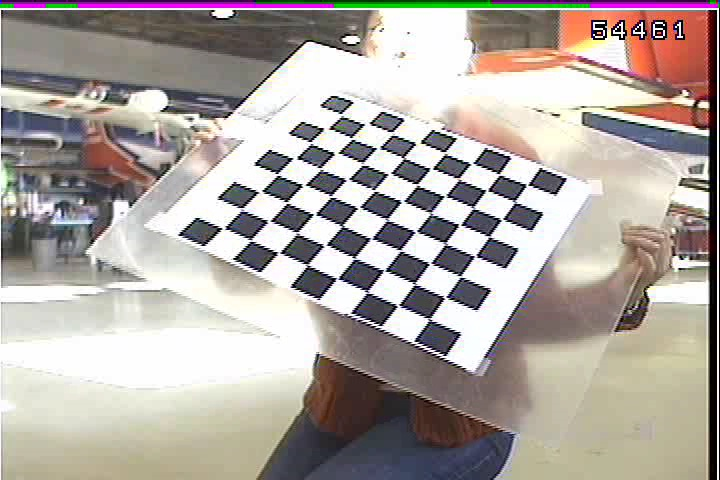
\includegraphics[width=4cm,keepaspectratio=true]{./Figures/camcal/camcal1_240.jpeg}
  \caption{A Subset of Camera Calibration Inputs}
  \label{fig:camcal}
\end{figure}

The program ``calibration.exe'' was used to calibrate the camera. This program came with the OpenCV installation. The digitized images have a resolution of 720 pixels in width and 480 pixels in height. Table \ref{tab:camcalresult} below listed the calibration results.

\begin{table}[h]
\caption{Camera Calibration Result}
\label{tab:camcalresult}
\centering
\begin{tabular}{|c|c|}
\hline
Parameter & Result\\ \hline
$f_x$ & 887.6 pixels \\ \hline
$f_y$ & 805.7 pixels\\ \hline
$c_x$ & 381.8 pixels\\ \hline
$c_y$ & 293.7 pixels\\ \hline
$k_1$ & -0.102 \\ \hline
$k_2$ & -0.535 \\ \hline
$p_1$ & 1.15e-003 \\ \hline
$p_2$ & 8.40e-003 \\
\hline
\end{tabular}
\end{table}
\FloatBarrier

\section{Data Preparation}
% word checked.
\subsection{Ground Truth Data Collection}
The localization ground truth data were obtained through the flight
control unit GS-111m on board the SUAS. The unit recorded the SUAS
position in GPS longitude and latitude coordinate. Orientation was
obtained from the roll pitch and heading measurements. Roll and pitch
accuracy has $0.1^\circ$ and $0.1^\circ$ in standard deviation.
Heading accuracy can achieve $0.5^\circ$ \cite{_athena_????}.

Landmark position ground truth came from digital elevation map (DEM)
downloaded from CGIAR-CSI website \cite{_cgiar-csi_????}. The DEM
contains longitude, latitude and sea level elevation of the terrain
with a resolution approximately 100 meters by 100 meters. 

%consider adding the ground truth DEM figure here. 

\subsection{Data Preparation}
To compare the estimated UAV poses and landmark position to the ground
truth, all data must be referenced to the same coordinate frame. For
ease of viewing, the reference frame used for data analysis is the
world frame defined by the first camera poses at time 0. 

The longitude and latitude of the SUAS position were first converted
to UTM using the WGS84 world geodetic system \cite{_world_????}. Many
software are readily available to do the conversion by taking GPS
coordinate and zone number as input. The software used in this work is
a python interface to PROJ.4 library \cite{_pyproj_????} called pyproj
\cite{_pyproj_????}. Secondly, in UTM coordinate, the ground truth of
the SUAS poses were brought to the world frame by subtracting their
value at time 0. The superscript Nav indicates that the value came
from the navigation measurement.

$$\text{True SUAS position}^W = 
Q_{step2}^{-1}Q_{step1}^{-1} \cdot\text{SUAS position}^{Nav}$$

\noindent where $Q_{step1}^{-1}$ and $Q_{step2}^{-1}$ is the inverse
transformation matrix for a reference frame evolving from UTM to world
frame. Detail formulation for coordinate transformation was given in
appendix \ref{ch:appendix1}. The UTM to world frame transformation is
illustrated in figure \ref{fig:utm_to_world}, and the transformation
parameters for step 1 and step 2 are listed below.

\begin{figure}[h]
  \centering
  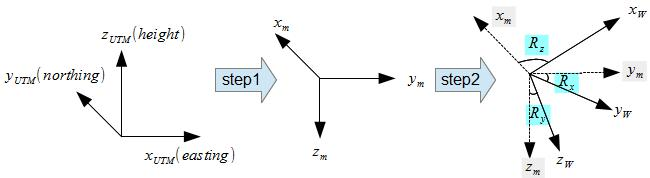
\includegraphics[width=12cm,keepaspectratio=true]{./Figures/utm_to_world.jpg}
  \caption{Coordinate transformation from UTM to world frame}
  \label{fig:utm_to_world}
\end{figure}

$$T_{step1} = \begin{bmatrix}Easting_{init}, Northing_{init},
  Height_{init}\end{bmatrix}$$
$$R_{step1} = \begin{bmatrix}180^{\circ}, 0^{\circ},
  -90^{\circ}\end{bmatrix}$$
$$T_{step2} = \begin{bmatrix}0, 0, 0\end{bmatrix}$$
$$R_{step2} = \begin{bmatrix}Roll_{init}, Pitch_{init},
  Azimuth_{init}\end{bmatrix}$$

\noindent where $Easting_{init}$, $Northing_{init}$ and
$Height_{init}$ are the SUAS's position in UTM when first image frame
was captured. 

SUAS orientation were represented in aircraft principle axes. This is
the case for both ground truth and estimated data. For the ground
truth to compare to the estimated data, the orientation at filter
initialization ($1^{st}$ image frame) was subtracted. 
$$\text{True SUAS orientation} =
\text{Orientation}^{Nav} - \text{Orientation}^{Nav} \text{at Initialization}$$

The estimated SUAS poses can be obtained from the world reference
frame estimates in the filter state vector:

$$ \text{Estimated SUAS poses} = 
[-O_{XYZ}^{C}, -W_{XYZ}^{C}]$$.


To compare landmark position, DEM data were converted into world frame
following the same procedure as the SUAS position. Landmarks estimated
from the CC\_EKF\_SLAM algorithm were converted to world frame using
the estimated SUAS localization results for reference frame evolving
parameters. Let $[X_i^W,Y_i^W, Z_i^W]^T_k$ be the $i^{th}$ landmarks
coordinates in world frame at step $k$, then

\begin{equation}
  \left[ \begin{array}{c}
    X_{i}^{W}  \\
    Y_{i}^{W}  \\
    Z_{i}^{W}  \\
  \end{array} \right]_k=Q^{-1}(\mathbf{O_{XYZ, k}^{c}}, \mathbf{W_{XYZ,k}^{c}})\left(\left[
    \begin{array}{c}
      x_{i}^{C} \\
      y_{i}^{C} \\
      z_{i}^{C} \\
    \end{array}
  \right]_k+\frac{1}{\rho _{i,k}}\mathbf{m}(\varphi_{i,k}^{C},\theta_{i,k}^{C})\right)
\end{equation}


%%% Local Variables:
%%% mode: latex
%%% TeX-master: "thesis.tex"
%%% End:
